\documentclass[tikz,border=12pt]{standalone}
\usepackage[T1]{fontenc}
\usepackage{mathpazo}
\usepackage{amsmath,amssymb}
\usetikzlibrary{arrows.meta, calc}

\definecolor{stblue}{HTML}{7B97AD}
\definecolor{rwgold}{HTML}{B8995E}
\definecolor{sage}{HTML}{7A9A7E}
\definecolor{dkbrown}{HTML}{3D3530}
\definecolor{wmgray}{HTML}{7B7067}
\definecolor{cream}{HTML}{F9F6F0}
\definecolor{border}{HTML}{D4C9B8}
\definecolor{terracotta}{HTML}{C47A6A}
\definecolor{lavender}{HTML}{907EA0}

\begin{document}
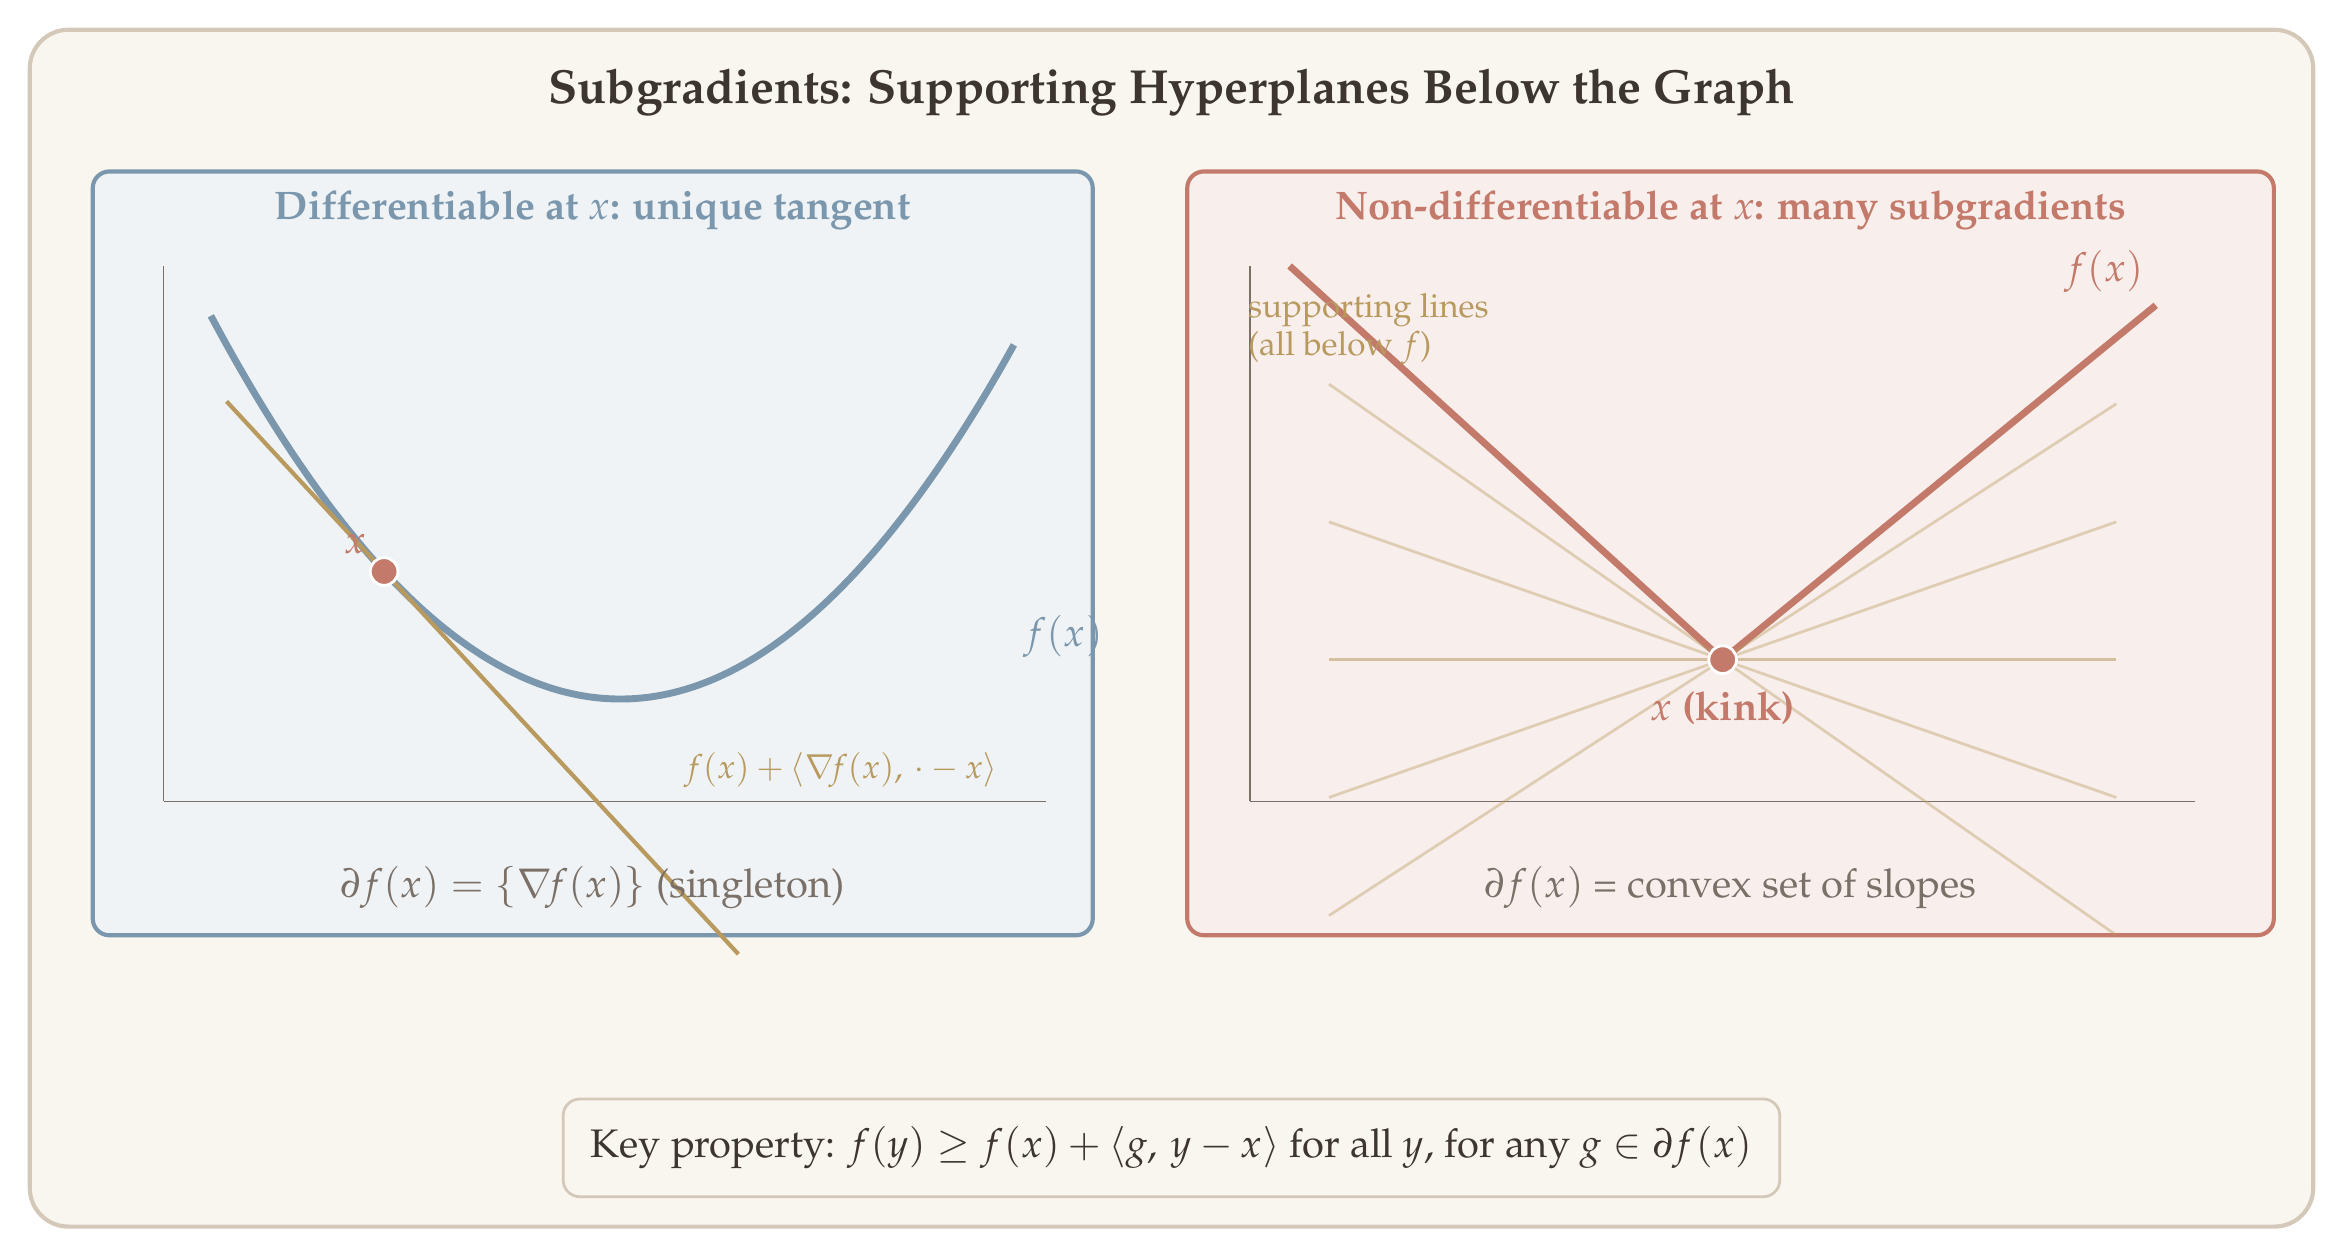
\begin{tikzpicture}[>={Stealth[length=4mm, width=3mm]}]

% Background
\fill[cream, rounded corners=14pt] (-0.5,-2.2) rectangle (28.5,13.0);
\draw[border, line width=1.5pt, rounded corners=14pt] (-0.5,-2.2) rectangle (28.5,13.0);

% Title
\node[text=dkbrown, font=\LARGE\bfseries] at (14.0,12.2)
  {Subgradients: Supporting Hyperplanes Below the Graph};

% ================================================================
% LEFT PANEL: Differentiable — unique tangent
% ================================================================
\fill[stblue!12, rounded corners=6pt] (0.3,1.5) rectangle (13.0,11.2);
\draw[stblue, line width=1.5pt, rounded corners=6pt] (0.3,1.5) rectangle (13.0,11.2);
\node[text=stblue, font=\Large\bfseries] at (6.65,10.7)
  {Differentiable at $x$: unique tangent};

% Axes
\draw[wmgray, line width=0.6pt] (1.2,3.2) -- (12.4,3.2);
\draw[wmgray, line width=0.6pt] (1.2,3.2) -- (1.2,10.0);

% Smooth convex curve: f(t) = 0.18*(t-7)^2 + 4.5
% At t=7: f=4.5, f'=0
% At t=4: f=0.18*9+4.5=6.12, f'=0.36*(4-7)=-1.08
% Tangent point at t=4: y=6.12, slope=-1.08
\draw[stblue, line width=2.5pt, smooth, samples=60, domain=1.8:12.0]
  plot (\x, {0.18*(\x-7)*(\x-7) + 4.5});
\node[text=stblue, font=\Large, right] at (12.0,5.3) {$f(x)$};

% Tangent point at t=4: f(4)=6.12, f'(4)=-1.08
\pgfmathsetmacro{\tx}{4.0}
\pgfmathsetmacro{\ty}{0.18*(\tx-7)*(\tx-7) + 4.5}
\pgfmathsetmacro{\tslope}{0.36*(\tx-7)}

% Tangent line: y = ty + tslope*(x - tx)
\draw[rwgold, line width=1.5pt, domain=2.0:8.5]
  plot (\x, {\ty + \tslope*(\x-\tx)});

% Point
\fill[terracotta] (\tx, \ty) circle (5pt);
\draw[white, line width=1pt] (\tx, \ty) circle (5pt);
\node[text=terracotta, font=\Large\bfseries, above left=3pt] at (\tx, \ty) {$x$};

% Tangent line label (below the line, in open space)
\node[text=rwgold, font=\large] at (9.8,3.6)
  {$f(x) + \langle \nabla\!f(x),\, \cdot - x \rangle$};

% Label
\node[text=wmgray, font=\Large, align=center] at (6.65,2.1)
  {$\partial f(x) = \{\nabla\!f(x)\}$ (singleton)};

% ================================================================
% RIGHT PANEL: Non-differentiable — many subgradients
% ================================================================
\fill[terracotta!12, rounded corners=6pt] (14.2,1.5) rectangle (28.0,11.2);
\draw[terracotta, line width=1.5pt, rounded corners=6pt] (14.2,1.5) rectangle (28.0,11.2);
\node[text=terracotta, font=\Large\bfseries] at (21.1,10.7)
  {Non-differentiable at $x$: many subgradients};

% Axes
\draw[wmgray, line width=0.6pt] (15.0,3.2) -- (27.0,3.2);
\draw[wmgray, line width=0.6pt] (15.0,3.2) -- (15.0,10.0);

% V-shaped function: kink at (21.0, 5.0)
% Left arm: slope -1.0, Right arm: slope +0.9
\draw[terracotta, line width=2.5pt] (15.5,10.0) -- (21.0,5.0) -- (26.5,9.5);
\node[text=terracotta, font=\Large, above left=1pt] at (26.5,9.5) {$f(x)$};

% Multiple supporting lines through the kink at (21.0, 5.0)
% slopes between left arm (-0.9) and right arm (+0.8)
\foreach \s/\op in {-0.7/0.4, -0.35/0.4, 0/0.55, 0.35/0.4, 0.65/0.4} {
  \draw[rwgold, line width=1pt, opacity=\op]
    (16.0, {5.0+\s*(16.0-21.0)}) -- (26.0, {5.0+\s*(26.0-21.0)});
}

% Kink point (on top of lines)
\fill[terracotta] (21.0,5.0) circle (5pt);
\draw[white, line width=1pt] (21.0,5.0) circle (5pt);
\node[text=terracotta, font=\Large\bfseries, below=8pt] at (21.0,5.0) {$x$ (kink)};

% Fan annotation (upper-left, away from lines)
\node[text=rwgold, font=\large, align=left] at (16.5,9.2)
  {supporting lines\\(all below $f$)};

% Label
\node[text=wmgray, font=\Large, align=center] at (21.1,2.1)
  {$\partial f(x)$ = convex set of slopes};

% ================================================================
% Bottom formula box
% ================================================================
\node[text=dkbrown, font=\Large,
      fill=cream, inner sep=10pt,
      draw=border, line width=1pt, rounded corners=6pt]
  at (14.0,-1.2)
  {Key property: $f(y) \geq f(x) + \langle g,\, y - x \rangle$
   for all $y$, for any $g \in \partial f(x)$};

\end{tikzpicture}
\end{document}
